\documentclass{article}
\usepackage{amsmath}
\usepackage{graphicx}
\bibliographystyle{IEEEtran}
\usepackage{caption}
\usepackage{subcaption}
\usepackage[colorlinks=true]{hyperref}
\title{Author Response to Reviewers for the paper `Eliminating prior-bias from sparse-projection tomographic reconstructions'}
\begin{document}
\maketitle

\textbf{Organization of this response:} We would like to thank the editor and all three reviewers for their insightful comments. Here, we are including our response to each reviewer, and pointers to modifications (suggested by the reviewers and the AE) in our revised manuscript.  Where necessary, we tie up related comments from the multiple reviewers for ease of understanding.  We have organized this document in three parts (a) Response to comments from AE (Section A), and (b) Response to significant points made by all the other reviewers (c) Detailed  responses to the comments of each of the reviewers.

To the best of our knowledge, we have painstakingly addressed each and every point of all the reviewers, and responded adequately.  We request the reader's time to go through our responses.

In some cases, we provide results in this document to justify our stand, but these same results are not in the updated manuscript, primarily because these results do not enhance the claims in our paper . In most other cases, we have shifted such results to supplementary material and have referred to them in this document.

For ease of understanding, since the current version of the manuscript is considerably reorganized, in this document, we have used the (longer) term ``Figure x'' to refer to a figure in the old version and ``Fig. x'' to refer to the related figure in the current version. Similarly, we have used the term ``Equation y'' to refer to an equation in the old version, and ``Eq. y'' to refer to an equation in the new version, and ``Table y'' to refer to a table in the old version and ``Tab. y'' to refer to a table in the new version. 

\section{Associate Editor comments}
(We have numbered the original review comments as AE-Cx, and italicized for clarity)

Two of the reviewers have raised some serious concerns about the paper, including one reviewer who opines that this work is not suited for publication in the transactions in its current form. While these concerns are sufficiently serious to merit a negative decision, I have decided to give the authors an opportunity to revise the manuscript so that they may address the constructive comments of the reviewers carefully and thoroughly followed by another round of review to assess the manuscript. In addition to the reviewer specific comments, please pay specific attention to the following:\\

\textcolor{blue}{\textbf{AE-C1.}\textit{ Overall organization of the paper to improve the exposition.}}

\textbf{Response:} 
We have now made the following significant changes in the organization of the paper:
The introduction has been modified and the stage set for outlining our contributions have been made.  We have replaced the earlier Figure 1 (which did not have longitudinal data) with a more appropriate figure (Fig.1). The unfamiliar terms ``unselective'' and ``selective'' prior have now been replaced by ``uniform'' prior and ``spatially varying'' prior to better communicate the property of the respective priors.
A new section  (Section 2) named ``Related Work'' has been included separately to contrast this work with the prevailing work in the literature. 
Details of the datasets have been moved to a separate section (Section 4) so the ground is properly set.
The two earlier sections: methods and results sections have now been split into the following 4 sections. This ensures better readability and emphasizes the cases where both uniform prior and spatially-varying prior are useful.
\begin{itemize}
 \item Section 6: Uniform prior-based reconstruction
 \item Section 7: Results: Reconstruction by uniform prior
 \item Section 8: Spatially varying prior-based reconstruction
 \item Section 9: Results: Reconstruction by spatially varying prior
   \end{itemize}
For greater clarity, we have now removed Schematic 1 (as suggested by R1) from the paper. We have  ensured that the rest of the paper can be followed without it. We have also moved the discussion on the earlier patch-based methods to supplementary material. However, results not reported earlier prior to this submission using the uniform prior on 3D volumetric data continues to be present (as mentioned above) in Section 6 since it forms an important part of our story for this paper.\\

\textcolor{blue}{\textbf{AE-C2.}\textit{ Highlight clearly the novelty of the presented work and provide accurate comparisons to relevant algorithms in the case when one has access to prior scans.}}

\textbf{Response:} We have now re-written the contributions section (Sec.3 of the main paper), that highlights the novelty of our work.  
As a response to the comparisons required,  in many cases, our methods are incomparable to previous algorithms because of the nature of the longitudinal study  We discuss this in the related work section. Further we reiterate that in our earlier manuscript version, we had compared our method with l1-regularized least squares (l1-ls) and FDK for 3D reconstructions. We had also compared (Fig.8) our method with many other iterative methods such as (ART, SART and SIRT) -- this set of comparisons was buried in a footnote, and perhaps not easily visible.
In addition to these, we now have included Table 3 to show a quantitative comparison of SSIM values of the reconstruction by various methods shown in Fig.8.  We also discuss compressed sensing (see AE-C3) results.
In addition, 
R3 has referred to ``Region-based iterative reconstruction of Structurally Changing Objects in CT''. This reference is now mentioned in our related work; although this paper is not directly applicable in longitudinal studies where object-priors `are' available, there is a reference in this paper to another paper which does make use of object-prior. We show how our work is superior in our response to R3 below (we include this in the supplementary material). \\

\textcolor{blue}{\textbf{AE-C3.}\textit{Discuss the compressed sensing methods used since there are several works on model-based iterative reconstruction/regularized inversion/CS type methods for CT.}}

\textbf{Response:} We believe we now have clearly brought out the compressed sensing based works both in the introduction and in the related work section.  Related points w.r.t. CS-type reconstruction made by R1/R3 appears below in B1 (and elsewhere in even greater detail).

In summary, we believe that the extensive work we have done based on the reviewer comments, while still maintaining the intellectual contributions of the original submitted version lends itself to the paper being accepted.

\section{Broad response to all reviewers}

We believe it is useful to single out the most serious criticism to this paper, and we wish to defend our stand. At this time, we request the reviewers  to kindly look at the first few sections, with slightly modified terminology (compared to the submitted version)  before continuing on to the responses. 

\begin{itemize}
  \item R1 and R3 are concerned about the blurring and over-regularized nature of the compressed sensing-based images.  In particular R3 is seriously concerned about the quality of Compressed Sensing reconstruction. Our response is that this is a function of the number of views. In short, if the number of views is sub-Nyquist, yes, indeed CS can provide good quality reconstruction, especially with the tuning method suggested by R1. (Our updated figures demonstrate this). 
However,  coming to the main contribution of the paper, if the number of views becomes significantly small (when compared even to sub-Nyquist), reconstructions using CS is less than satisfactory, despite the removal of sub-sampling artefacts. This has also been pointed out earlier in a different (not ours) published work [11], Page 4, line 22.  We have now described the use-case for CS reconstructions in Fig. 1 and have elaborated on the blurred artefacts in our  response in R3-C7.
\item All reviewers are concerned about the seemingly low SSIM value (relatively poor reconstruction) for one of the experiments.  (Figure 10-c in the original document) while results in all the other experiments are acceptable to prove the point.  For instance R2 says ``I have one main question concerning Table 1, where I notice FDK gives for the ROI much better SSIM value than the variants of the proposed method.''  
Of course, we never intended to *not* mention this, which is why it was picked up very easily by all the reviewers, and in real life situations, it is unreasonable to expect that the ROI of detailed changes is known in advance. 

In response, we first note that our updated results of comparison for this dataset (after the tuning suggested by R1) *now* results in a favourable result (Table 3).  That said, we agree that the FDK reconstructions can be superior, as evidenced for this particular dataset alone -- presumably when the region of interest is known a-priori (which is not always the case). We have devoted a separate section in the `Discussion' for this particular concern: Tab.8 better explains why our method is suitable, and Fig. 19(e) the more pleasing visual result.  
\item R1 and R3 also raise another significant point:  What happens if we have only the object prior term and ignore the sparsity prior?.  This indeed is relevant. Our response is that the answer to the question revolves around the quality of the prior. In our experiments, the object priors are of high quality, the number of views very few (the title of our paper), and hence the object-prior has a dominant effect when compared to sparsity prior;  adding the sparsity prior improves the reconstruction marginally.  That said, ignoring the sparsity prior would be akin to ignoring the established work revolving around compressed sensing.  If the object-priors were of poor quality, or if the number of views (still sub-Nyquist) were to be increased from our very few views, then the sparsity term will start playing a part.  
\item R3 remarks that `it's simply not true' about some of the overarching broad statements which we had claimed in our earlier submission (for example, ``in most of the literature on tomographic reconstruction, the results are shown on reconstruction from projections simulated from 3D volumes''). In our current version, we have now either given better context to such statements or have retracted our misunderstandings with the wisdom in R3's remarks.
\end{itemize}

\section{ Detailed response to individual review comments}

\subsection{Response to Reviewer 1}
There are some concerns associated with the compressive sensing (CS) method, the explanation for weight selection, and the clarity of results. Some of the major issues are described below. 

\textcolor{blue}{\textbf{R1-C1:}\textit{In Fig. 4, the caption says CS and no prior. This is not true. CS does have a prior in the sense that it forces the reconstruction to lie in a sparse basis. You did explain this aspect of CS in section III (A).}}

\textbf{Response:} Agreed.  CS does use the sparsity prior. We have now moved this point much earlier in the introduction, and point out some of the advantages of using object-prior. Sec.1, Page1. We have corrected the captions. Specifically, (for example) the earlier caption of Fig.4-c: ``CS and no prior resulting in blurred bone structures'' has now been replaced by ``l1-ls resulting in blurred bone structures''. In the latter, ``l1-ls'' refers to L1-regularized least squares optimization \\

\textcolor{blue}{\textbf{R1-C2:}\textit{$\lambda_1$ seems to decide the strength of the CS prior. However, in section V (B), you mention that $\lambda_1$ is always chosen to be one. But, it is clear that the potato image in Fig. 10 (c) is over-regularized. It is extremely blurred.}}

\textbf{Response:} Agreed. See response is \textcolor{blue}{\textbf{R1-C3}}.\\

\textcolor{blue}{\textbf{R1-C3:}\textit{ In CS, since you use cross-validation on a test image to select $\lambda_1$, it is necessary to tune this parameter until you reach a desired SSIM or root-mean-squared-error (RMSE). With CS priors, I would expect increasing $\lambda_1$ to also lead to smoother results.}}  

\textbf{Response:} With respect to Figure. 10(c) of the submitted paper which corresponds to Fig.17(c) of the new version, we have now updated the reconstruction after tuning $\lambda_1$ to get the optimal result for l1-ls, as suggested by Reviewer 1. The optimal $\lambda_1$ was found to be 1.7. 

In Sec.5 of our supplementary material, we describe why the image in Fig.17(c) (Fig.10(c) of the old version) appears over-regularized by presenting reconstructions on 2D potato dataset for different number of views and optimally tuned $\lambda_1$ values.   \\

\textcolor{blue}{\textbf{R1-C4:}\textit{ What is the sparsity basis for CS prior in equation (1)? }}

\textbf{Response:} We have chosen DCT as the sparsity basis, and have now clarified this in the paper. We had observed that there is no significant improvement if, say, the wavelet transform were instead used as the basis.\\

\textcolor{blue}{\textbf{R1-C5:} \textit{Why is a CS prior necessary when you have the selective/unselective prior? What happens if there is no CS prior and if we use only the selective/unselective priors?}}

\textbf{Response:} Although the data-agnostic CS/sparsity  prior and the data-dependent object-prior  (either uniform or spatially varying) affect independent terms in the overall cost function (Eq.6), best results are obtained when both the priors are used together. Whether to use the CS prior or not is a function of the quality of the object-prior. In our case, the object priors are of high quality, and hence the object-prior has a dominant effect. Adding sparsity prior improves the reconstruction marginally.\\

\textcolor{blue}{\textbf{R1-C6:}\textit{Schematic 1 in section III (B) does not make sense. But, the explanation in section III (B) (2) is clear.}}

\textbf{Response:}  For greater clarity, we have now removed Schematic 1 from the paper; We have  ensured that the rest of the paper can be followed without it.\\

\textcolor{blue}{\textbf{R1-C6(b):}\textit{found section III (B) (2) algorithm to compute weights map W very interesting. However, it is hard to understand what artifacts can be attributed to the system geometry and an algorithm. For instance, in the third step, you mention that the difference between $P^{fdk}$ and $X^{fdk}$ will not contain false positives due to imaging geometry but will contain false positives specific to the reconstruction method. Can you show these artifacts for the potato dataset? While Fig. 7 showing weights is interesting, from a clarity standpoint, I would like to see images of artifacts that get removed at each stage of your algorithm (2) Algorithm to compute weights maps W.}}

\textbf{Response:} To illustrate how different reconstruction methods lead to different artefacts and how combining them carefully can cancel those artefacts, we present a few intermediate weights maps for a 2D reconstruction from 12 views (of the test image in Fig.10 of the paper), with and without noise. Due to the lack of space, we have not included the below images in the main paper.
%-----------------------------potato data
\begin{figure}[!h]
    \begin{subfigure}[b]{0.24\linewidth}
        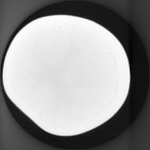
\includegraphics[width=\textwidth]{../images/potato/template_1.png}
\captionsetup{labelformat=empty}       
 \caption{}
    \end{subfigure}
    \begin{subfigure}[b]{0.24\linewidth}
        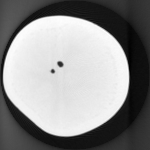
\includegraphics[width=\textwidth]{../images/potato/template_2.png}
\captionsetup{labelformat=empty}
        \caption{}
     \end{subfigure}
    \begin{subfigure}[b]{0.24\linewidth}
        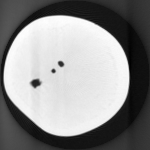
\includegraphics[width=\textwidth]{../images/potato/template_3.png}
\captionsetup{labelformat=empty}
        \caption{}
     \end{subfigure}
    \begin{subfigure}[b]{0.235\linewidth}
        \fcolorbox{yellow}{yellow}{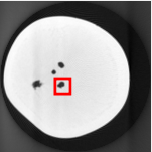
\includegraphics[width=\textwidth]{../images/potato/testIm_color.png}}
\captionsetup{labelformat=empty}
        \caption{}
\label{fig:potato_test}
     \end{subfigure}
      \caption{Potato dataset: One slice each from the previously scanned objects (the first three from left) and a slice from the test 
        volume (extreme right). Notice the appearance of the fourth
        hole in the test slice. }
\label{fig:object-prior_test_potato_A1}
\end{figure}


In the Figs.~\ref{fig:weights_no_noise} and~\ref{fig:weights_with_noise}, notice how the weights map is different for each of the methods and how it is improved when it is computed using two or more methods. We observe similar benefits even in the presence of small quantities of noise as shown below. 

In the actual reconstruction of the images, the prior term is well represented and these effects are not immediately visible.  However, with low quality priors the effects may be visible.

\newpage
\textbf{Case 1: No noise in projections:}
\begin{figure}[!h]
    \begin{subfigure}[b]{0.19\linewidth}
        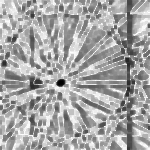
\includegraphics[width=\textwidth]{../images/potato/artefacts/no_noise/weightsIm_fbp30.png}
\captionsetup{labelformat=empty}       
 \caption{FBP}
    \end{subfigure}
    \begin{subfigure}[b]{0.2\linewidth}
        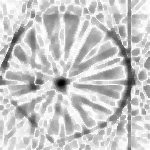
\includegraphics[width=\textwidth]{../images/potato/artefacts/no_noise/weightsIm_sirt30.png}
\captionsetup{labelformat=empty}
        \caption{SIRT}
     \end{subfigure}
    \begin{subfigure}[b]{0.2\linewidth}
        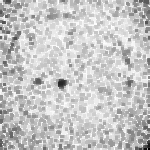
\includegraphics[width=\textwidth]{../images/potato/artefacts/no_noise/weightsIm_sart30.png}
\captionsetup{labelformat=empty}
        \caption{SART}
     \end{subfigure}
    \begin{subfigure}[b]{0.2\linewidth}
        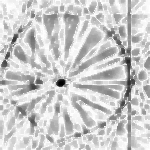
\includegraphics[width=\textwidth]{../images/potato/artefacts/no_noise/weightsIm_fbp_sirt30.png}
\captionsetup{labelformat=empty}
        \caption{FBP + SIRT}
    \end{subfigure}
    \quad
        \begin{subfigure}[b]{0.2\linewidth}
        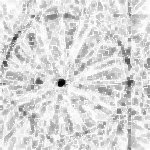
\includegraphics[width=\textwidth]{../images/potato/artefacts/no_noise/weightsIm_fbp_sart_sirt30.png}
\captionsetup{labelformat=empty}
        \caption{FBP + SART + SIRT}
     \end{subfigure}
      \caption{Weights images by various methods while reconstructing the test in Fig.~\ref{fig:object-prior_test_potato_A1} from 12 views and no noise}
\label{fig:weights_no_noise}
\end{figure}

\textbf{Case 2: Noise with 0 mean and SD = 1$\%$ of the mean of the measurements}
\begin{figure}[!h]
    \begin{subfigure}[b]{0.2\linewidth}
        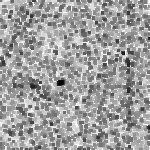
\includegraphics[width=\textwidth]{../images/potato/artefacts/with_noise/weightsIm_fbp30.png}
\captionsetup{labelformat=empty}       
 \caption{FBP}
    \end{subfigure}
    \begin{subfigure}[b]{0.2\linewidth}
        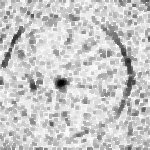
\includegraphics[width=\textwidth]{../images/potato/artefacts/with_noise/weightsIm_sirt30.png}
\captionsetup{labelformat=empty}
        \caption{SIRT}
     \end{subfigure}
    \begin{subfigure}[b]{0.2\linewidth}
        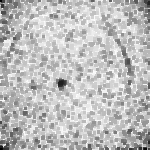
\includegraphics[width=\textwidth]{../images/potato/artefacts/with_noise/weightsIm_sart30.png}
\captionsetup{labelformat=empty}
        \caption{SART}
     \end{subfigure}
    \begin{subfigure}[b]{0.2\linewidth}
        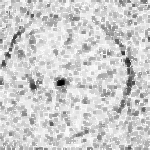
\includegraphics[width=\textwidth]{../images/potato/artefacts/with_noise/weightsIm_fbp_sirt30.png}
\captionsetup{labelformat=empty}
        \caption{FBP + SIRT}
    \end{subfigure}
    \quad
        \begin{subfigure}[b]{0.2\linewidth}
        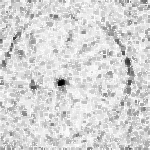
\includegraphics[width=\textwidth]{../images/potato/artefacts/with_noise/weightsIm_fbp_sart_sirt30.png}
\captionsetup{labelformat=empty}
        \caption{FBP + SART + SIRT}
     \end{subfigure}
      \caption{Weights images by various methods while reconstructing the test in Fig.~\ref{fig:object-prior_test_potato_A1} from 12 views in the presence of noise.}
\label{fig:weights_with_noise}
\end{figure}

\textcolor{blue}{\textbf{R1-C6:}\textit{ In results, the images are simply too big relative to the ROIs, which are tiny. It is very difficult to see the changes within the ROI. If the paper is printed, then there is no way to zoom into the images. It will be better if you could also present zoomed images of the ROI. Otherwise, you could present one full sized image and rest of the images could be only the ROI. }}

\textbf{Response:} While the zoomed-in RoI of Okra is in Figure 13 of the old manuscript (Fig.14 of the new manuscript), the zoomed-in RoI of the sprouts dataset has now been added in Fig. 16.  For other cases, larged sized images are in the supplementary material.\\

\textcolor{blue}{\textbf{R1-C7:}\textit{ Table I, II, and III present SSIM comparison. It will also be interesting to present a root mean squared error (RMSE) comparison. RMSE measure will help in evaluating the quantitative accuracy of your reconstruction.}}

\textbf{Response:} The optimal values of parameters obtained by tuning RMSE were found to be different from those obtained by tuning SSIM. Hence, for consistency, we choose only one metric (SSIM) to report accuracy of all reconstructions.
Moreover, SSIM gives us the flexibility to measure the fidelity of the structural content of our reconstruction with respect to that of test volume.\\ 

\textcolor{blue}{\textbf{R1-C8:}\textit{ For instance, in Fig. 10 (e), the region within the ROI seems to be brighter than the surrounding holes. This may also happen if an incorrect choice of the CS prior regularization parameter $\lambda_1$ results in excessive blurring.}}
  
\textbf{Response:} Despite tuning $\lambda_1$, In Fig. 19(e) (previously Fig.10(e) of the old version), the information about the new region (within RoI)  is present only in the measurements of the test, and is absent in all of the templates. This is unlike the case for the surrounding holes, the information about which is present both in the measurements of the test and the templates. Hence, the reconstruction of the hole in the RoI is not as sharp as the other holes.\\

\textcolor{blue}{\textbf{R1-C9:}\textit{Some relatively minor issues are below- Page 3, line 7, section II: Consider defining longitudinal study.}}
  
\textbf{Response:} We have now defined longitudinal study in the paper (Sec. 1). Longitudinal studies here refers to the acquisition of sequential CT scans of the same subject to track time-evolving changes within the subject's interior.  \\

\textcolor{blue}{\textbf{R1-C10:} \textit{Images in Fig. 3 seem to be clipped in the lower left along a circular arc! Are all reconstructions within a circular outer region of interest?}}

\textbf{Response:} All the reconstructions are within the circular region for this dataset. The ground-truth for this dataset consists of reconstructions from a proprietary software used in the CT machine at the Tata Memorial Hospital, Mumbai. The  RoI was chosen by the proprietary software and hence the exact reason for its choice is known only to the vendors. Based on inputs from physicians at the Centre, we have ensured that the RoI indeed encompasses the regions of interest, i.e. the organ in which ablation is being performed.\\


\textcolor{blue}{\textbf{R1-C11:}\textit{In Fig. 8, what is (g) combined? Also, there is no (h) but is mentioned in caption.}}

\textbf{Response:} The caption has now been correctly renamed to (g). 
By `combined', we denote the weight map computed as per Eq.7.  This equation incorporates the use of the eigen-space of the templates reconstructed from various methods (such as ART, SART, SIRT, etc.), and pilot reconstructions of the test,  again reconstructed from various methods. In Eq.7, the min(.) operator ensures that we select the new regions that are unanimously detected by all the methods of reconstruction. Hence, the word `combined' denotes that all the reconstruction methods are combined to give information about the new regions of the test.\\

\textcolor{blue}{\textbf{R1-C12:}\textit{ Try to mention the actual number of views/projections instead as a percentage. The percentage only makes sense when you are comparing against Nyquist limit for views. For instance, the total number of views for Potato dataset is 900, which is simply too many for a reconstruction size of 150x150. For such a small reconstruction, 900 is not a ``typical'' number views. It may be more ``typical'' to use 150 views in standard practice. So, expressing views as a percentage of 900 is confusing.}}
  
  \textbf{Response:} Just to clarify, as mentioned in the paper, the 900 views for the potato dataset was used to reconstruct the ground-truth 3D volume of size 150 x 150 x 100, and not a 2D slice of size 150 x 150.  Each of the projection images was of size 150 x 150.
  
Since our imaging method is circular cone beam projection, let us first assume a 2D example. Consider a circle of radius R=1 that envelops an unknown 2D region X. Then, the circumference of the circle in pixel units will be $2\pi R_p$, where$ R_p$ represents the radius in pixel units, i.e., the number of image-pixels that fit within the radius of the circle. Now, let us assume that we want to pass rays around a half of a circle (due to symmetry). We can reasonably assume that a set of $(2*\pi*R_p)/2$ angles will be ``sufficient'' to faithfully reconstruct X.
\begin{itemize}
\item Given size of the 2D object $= 200 x 200$, the length (in pixel units) of the diagonal of this image $= 200*\sqrt(2)$, and this is twice the radius of the enclosing circle.
\item Since our imaging method is circular cone beam projection, we assume a circle to tightly bound the object.
\item $R_p = 282.84/2 = 141.4$
\item No. of views $= 2*\pi*R_p = 888$ views
\end{itemize}

Similarly, in the case of 3D, assume the object is enclosed within a sphere of unit radius R. Let $R_v$ denote the radius in voxel units, i.e., number of object-voxels that fit within the radius of the sphere. Hence, in 3D, one way to compute sufficient number of views would be the following:
\begin{itemize}
\item Given size of the object scanned $= 150 x 150 x 100$, the length of the space diagonal of this cuboid = $\sqrt{(100^2 + 100^2 + 150^2)}$
\item Since our imaging method is circular cone beam projection, we assume a sphere tightly bounding the object.
\item The radius of this sphere in voxel units ($R_v$) will be $\sqrt{(100^2 + 100^2 + 150^2)}/2 = 103$
and, surface area of the sphere $= 4*\pi*(R_v)^2 = 133320$.
\item If we want to pass at least one ray for every surface voxel of this sphere, we will need 133320/2 (since sphere is symmetrical, and ray at 30 deg will pass through same voxels as ray at 30 +180 deg) = 66658 views. 
\end{itemize}
Hence our choice of 900 views for reconstruction of the ground-truth is not exceedingly large. It just happens to be sufficient due to the homogenous structure of the interior of the object (potato).

Since our gold-standard for measuring accuracy of our technique's reconstruction is the ground-truth reconstruction obtained from 900 views (for the potato dataset), we have measured our achieved reduction in views as a fraction of the views used for reconstructing ground-truth. \\

\textcolor{blue}{\textbf{R1-C13:}\textit{ Hard to notice the features within the ROI in Fig. 15. It may help to present images that zoom into the ROI.}}
    
\textbf{Response:} The zoomed-in RoI is now shown in Fig. 16. \\

\textcolor{blue}{\textbf{R1-C14:}\textit{ In section V (B), how was the cross-validation or empirical selection of $\lambda_1$ and $\lambda_2$ done? Did you use SSIM as a comparison metric? Did you use any particular object prior image for cross-validation? If so, which image did you use? }}

\textbf{Response:} In our earlier submission, $\lambda_1$ and $\lambda_2$ values were chosen by reconstructing the test volume by sweeping through a range of values and selecting the set of values that gave a reasonable visual quality. In the current version of the paper, we had first chosen $\lambda_1$ as that value which maximizes the SSIM of the l1-ls reconstruction. This value was retained for uniform and spatially-varying prior based reconstruction as well. $\lambda_2$ was chosen clairvoyantly,  i.e., based on the value that gave the best visual results on the test.\\

\textcolor{blue}{\textbf{R1-C15:}\textit{ You are allowed to submit documents or media as supplementary material. Instead of posting them on a dropbox, you could submit them as supplementary material to the journal. You could also use supplementary material to add additional text or figures to reduce number of pages in main paper.}}
    
\textbf{Response:} Thank you for the suggestion. We have now submitted the supplementary material  on the publication portal. \\

\textcolor{blue}{\textbf{R1-C16:}\textit{ To save space and if you feel comfortable, you could move the section III (A) (1) on patch based techniques to supplementary since it is not a contribution of your paper.}}
    
\textbf{Response:} In order to save space and for greater clarity, we have now moved the discussion on patch-based techniques to supplementary material.

\section{Response to Reviewer 2}
(We have numbered these comments as \textbf{R2-Cx}, and italicized for clarity)\\

\textcolor{blue}{\textbf{R2-C1.}\textit{ I have one main question concerning Table 1, where I notice FDK gives for the ROI much better SSIM value than the variants of the proposed method. What is the reason of this? Why can then the authors state that their method is better than FDK? A bit more detailed explanation would be satisfactory.}}

\textbf{Response:} We hypothesize that because the volume of this dataset (potato) is very homogenous (without intricate  structures), the test measurements capture sufficient information about the new regions even with $5\%$ views and hence FDK performs very well in the exact region of interest (shown as red RoI in Fig. 19(a)). However, as we expand the region of interest (green and cyan RoI in Fig. 19a), the prior-based methods perform better than FDK (please refer Table 8) in that they minimize the sub-sampling artefacts.  We have now discussed this in Section 8. B - ``Reconstruction of homogenous data''.
Had the new region been embedded within an intricate background (like the sprouts and okra), its reconstruction does give rise to artefacts as seen in Figs.13-b and 15-b. 

Beside this, I only have minor comments:\\

\textcolor{blue}{\textbf{R2-C2}\textit{. P1, L49, right panel: "a" should not be typeset in italic.}}

\textbf{Response:} The italicized `a' here is used to emphasize the selection of `any one' particular template amongst the many available ones. So, we retain the typeset on ``a'' and for greater clarity, italicize the word `particular' as well . The statement now reads:
``there is the key issue of choice of a particular previously scanned object among the many previously acquired scans.''\\

\textcolor{blue}{\textbf{R2-C3.}\textit{P2, L31, left panel: The subtitle should be typeset in bold.}}

 \textbf{Response:} Accepted. The typeset has been changed.\\

\textcolor{blue}{\textbf{R2-C4. }\textit{P2, L50, left panel: ``reconstruction-'' should be corrected to ``reconstruction -''}}

 \textbf{Response:} Accepted. This has been corrected.\\

\textcolor{blue}{\textbf{R2-C5.}\textit{P5, L10, left panel: ``Eq 6'' should be corrected to ``Eq. 6'' (same in P6, L54, right panel}}

 \textbf{Response:} Accepted. This has been corrected, and the equation has now been moved to  supplementary material (Eq.2). \\

\textcolor{blue}{\textbf{R2-C6.}\textit{ P6, L17, left panel: ``i.e'' should be replaced with ``i.e.'' (correct each further occurrence}}

 \textbf{Response:} As per the conventional use, ``i.e'' has now been replaced by ``i.e.,'' in all occurrences in the paper.\\

\textcolor{blue}{\textbf{R2-C7. }\textit{P6, L42, left panel: ``Eqn. 8'' should be corrected ``Eq. 8'' (same in P7, L19, left panel}}

  \textbf{Response:} Accepted. These have been corrected.\\
 
 \textcolor{blue}{\textbf{R2-C8.}\textit{ Caption of Fig. 8: The correct form is (a)-(f) and (g)}}

  \textbf{Response:} Accepted. This has been corrected.\\
 
 \textcolor{blue}{\textbf{R2-C9.}\textit{ P6, L40, right panel: Subtitle should be typeset in bold}}
 
  \textbf{Response:} Accepted. The typeset has been changed.\\

 \textcolor{blue}{\textbf{R2-C10.}\textit{ P7, L3, and L7: ``proposed methods'' <--> "proposed method". Choose one.}}
 
 \textbf{Response:} In Sec.6, we use ``Proposed method'' to refer to uniform prior-based method, and in Sec.8 we use ``Proposed method'' to refer to spatially varying prior-based method.\\

\textcolor{blue}{\textbf{R2-C11.}\textit{ Caption of Figs 10, 12, and 13: ``Unselective prior'' should be typeset in two lines instead of three.}}

  \textbf{Response:} Accepted. This has been typeset.\\

 \textcolor{blue}{\textbf{R2-C12.}\textit{ P7, L50, left panel: Replace ``Figs. 9'' with ``Fig. 9''}}
 
  \textbf{Response:} Accepted. This has been corrected.\\
 
 \textcolor{blue}{\textbf{R2-C13.}\textit{ P7, L28, right panel: do not use bold typesetting here}}
 
  \textbf{Response:} Accepted. This has been corrected.\\

 \textcolor{blue}{\textbf{R2-C14.}\textit{ Caption of Fig. 15: ``Letters missing''}}
 
  \textbf{Response:} Accepted. This has been corrected.\\

 \textcolor{blue}{\textbf{R2-C15.}\textit{ P8, L49, right panel: Correct ``shows'' to ``show''}}
 
 \textbf{Response:} Accepted. This has been corrected.\\

 \textcolor{blue}{\textbf{R2-C16.}\textit{ Caption of Fig. 16: ``slice-8'' should be replaced with ``image-8''}}
 
 \textbf{Response:} Accepted. This has been corrected.\\

 \textcolor{blue}{\textbf{R2-C17.}\textit{ P9, L20, right panel: Move [16] to the second place.   }}
 
 \textbf{Response:} Accepted. This had been corrected.\\

\textcolor{blue}{\textbf{R2-C18.}\textit{P9, L34, right panel: ``[38](FDK'' space is missing}}
 
 \textbf{Response:} Accepted. This has been corrected.\\

 \textcolor{blue}{\textbf{R2-C19.}\textit{P9, L36, right panel: ``in-dept'' should be corrected to ``in-depth'', ``in'' should be corrected to ``is''}}
 
 \textbf{Response:} Accepted. These have been corrected.\\

 \textcolor{blue}{\textbf{R2-C20.}\textit{ Caption of Fig. 17: ``weight maps'' should be corrected to ``weights maps''}}
 
\textbf{ Response:} Accepted. This has been corrected to `weights-maps' in all occurrences in the paper.\\

 \textcolor{blue}{\textbf{R2-C21.}\textit{ Acknowledgement: ``Dr.Andrew Kingston'' space is missing}}
 
\textbf{ Response:} Accepted. This has been corrected.      

\section{Response to Reviewer 3}
(We have numbered these comments as R3-Cx, and italicized for clarity)

\textcolor{blue}{\textit{This paper extends an existing algorithm for reconstructing longitudinal tomographic data with a reduced number of projections, by adding a weight map that determines how much to weigh a specific term in the cost function for each voxel of the reconstructed image. The authors give an explanation of the approach, and show results for both simulated and experimental data. Although the proposed approach seems mathematically sound, the paper itself has several significant issues that make it difficult to assess whether the approach actually improves on existing work. }}\\

\textcolor{blue}{\textbf{R3-C1:}\textit{ Most importantly, results are compared with only a single existing method that is specifically designed for low-angle tomography (compressed sensing), and the results of that method seem sub-optimal (at least, it does not match my experience with both applying such methods myself and published results of such methods). }}

\textbf{ Response:} The results of the (compared, CS) method are sub-optimal because of a significantly fewer number of views.  We show  (see R3-C7) that if we increase the number of views, CS actually does very well, as expected, and as mentioned by the reviewer.

We have compared our 2D reconstructions with many other iterative techniques such as SIRT, SART and ART, as seen in Fig. 12 (Figure.8). Earlier we had not included the SSIM values,  and these now appear in Tab. 3.  In addition, we have now performed a 2D reconstruction to compare our method with [3] (please see Sec. 7 of our supplementary material.)\\

\textcolor{blue}{\textbf{R3-C2:}\textit{ Since no details are given about the method that is compared with (what function does in optimize?}}

\textbf{ Response:} In our submitted paper, we had compared our method to the the standard filtered back projection (written as FBP in Figure 1), and CS sensing using l1-ls (e.g. Line 33, Column 2, Page 4). The function optimized was given in Equation 8. We agree that we should have mentioned this earlier in the description, and this has been taken care of in the revised document. 

Of the many other prior-based techniques, we have now discussed  below how we contrast with them in Sec.2 (`Related work'). In addition, we have now performed a 2D reconstruction to compare our method with [3]. In [3], the new changes are directly detected in the measurement space by computing the difference between the measurements of the test and the corresponding simulated measurements of the template. This difference-volume is then reconstructed and then fused (added to) with the original high quality template.
However, in the above method, the sub-sampling artefacts present in the difference-volume gets carried over to the final reconstructed image. This can be seen in the visual results (and quantitative comparison) in Sec. 7 of our supplementary material.\\


\textcolor{blue}{\textbf{R3-C3:}\textit{ what were the parameters? how were these chosen?), the experimental results in the paper give very little information to the reader.}}

\textbf{ Response:} Details of the parameters and their tuning were earlier discussed in Section 5B. $\lambda_1$ was set equal to 1 in all datasets (as observed by R1, and line 53, page 9, column 2).  THis was done by visual inspection for one of the dataset and used elsewhere as is. We had earlier mentioned that we are using DCT in Page 6 (right column, line 58). 

For greater clarity, we have now explicitly mentioned the DCT bases right at the beginning on page 1 Section 1 (Introduction, below Eq.1).  Further, we have now tuned $\lambda_1$ (as per R1's suggestions) to maximize SSIM of the whole reconstructed test-volume for l1-ls reconstruction of each dataset. Once the value was chosen, we retained the same $\lambda_1$ value for uniform prior and spatially-varying prior as well. However, this has only marginally improved the reconstructions over our previous ones in the earlier manuscript. Here below, we present the changes in the accuracies due to tuning of $\lambda_1$ in Tables~\ref{tab:sprouts_revised_ssim}, and~\ref{tab:okra_revised_ssim}.

The new visual results and SSIM values are in Figs. 13, 15 and 19, and in Tables 4, 5 and 8. 


\begin{table}[!h]
  \caption{Old and revised SSIM (within red RoI) for 3D sprouts dataset}
  \label{tab:sprouts_revised_ssim}
\begin{tabular}{|l|l|l|}
\hline
 & \textbf{Earlier reported SSIM} & \textbf{Revised SSIM} \\ \hline
\textbf{l1-ls} & 0.84 & 0.86 \\ \hline
\textbf{Uniform prior} & 0.83 & 0.83 \\ \hline
\textbf{Spatially varying prior} & 0.88 & 0.88 \\ \hline
\end{tabular}
\end{table}


\begin{table}[!h]
  \caption{Old and revised SSIM (within red RoI) for 3D okra dataset}
  \label{tab:okra_revised_ssim}
\begin{tabular}{|l|l|l|}
\hline
 & \textbf{Earlier reported SSIM} & \textbf{Revised SSIM} \\ \hline
\textbf{l1-ls} & 0.83 & 0.84 \\ \hline
\textbf{Uniform prior} & 0.85 & 0.85 \\ \hline
\textbf{Spatially varying prior} & 0.88 & 0.88 \\ \hline
\end{tabular}
\end{table}

\textcolor{blue}{\textbf{R3-C4:}\textit{ To address these issues, a large amount of changes would be required in the paper (not only in the experiments, but also throughout the paper, since the performance of compressed sensing methods is one of the main motivations of introducing a new approach). Other issues are present in the paper as well (see below for more detailed comments). Therefore, I unfortunately have to recommend rejection of the current manuscript.}}

\textbf{Response:} We have now made changes as per this comment and those of the Associate Editor; the details of these are given in our individual responses to the comments. In addition, here we wish to state that the performance of compressed sensing is not one of the main motivations of the paper. The use of uniform and spatially-varying object-priors in a longitudinal setting is the main contribution of this paper and these techniques are independent of the sparsity-prior (CS) being used, i.e., object-specific prior can be imposed even when $\lambda1$, the weight of sparsity prior, is set to $0$.  The success of our method on a real-life dataset in a clinical setting is a testament to our methods.\\

%\textbf{Detailed Comments}

\textcolor{blue}{\textbf{R3-C5:}\textit{ The comparisons with existing methods in the current manuscript are insufficient to support the conclusions made in the paper. My main concerns are: - The authors only compare with a single method specific to reconstructing tomographic images from a low number of projections (which they call compressed sensing). However, this topic is highly studied, and there are many methods available for this. The paper would be improved by including results from more methods, for example dictionary learning, total variation minimization, algebraic techniques (DART etcetera), or even simply SIRT with a nonnegativity constraint.}}

\textbf{Response:} This comment is similar to R3-C4. The main aim of our paper is the usage of an object-prior along with a weights map for reconstruction from highly undersampled projections in a longitudinal study. When the number of views is extremely small, then undersampling artifacts will affect any baseline method, be it SIRT, CS, ART or any other. However incorporation of object priors will significantly help to mitigate those artifacts.
In Fig.12 (Figure 8), we had earlier shown a visual comparison of 2D reconstructions of one of the datasets (potato) by all of the following methods: FBP, CS with DCT as sparsity prior, CS with Haar as sparsity prior, ART, SART, SIRT and our weighted prior method.
We have now also included a quantitative comparison of the accuracy of these results in Tab. 3 of the new manuscript.\\

\textcolor{blue}{\textbf{R3-C6:}\textit{ No details are given about the CS method that was compared with. What type of sparsity did the method assume? What objective function did it minimize? What parameters did the authors choose? How were those parameters chosen? How many iterations were used to minimize the objective function? Without this information, the comparison does not have much information, and therefore can't be used to support the conclusions made in the paper.}}

\textbf{Response:} This is similar to R3-C3. We had earlier mentioned that we are using DCT in Page 6 (right column, line 58). For greater clarity, we have now mentioned this in Section 1 (Introduction, below Eq.1).
The objective function minimized while using l1-ls (CS) optimization is now introduced in Eq.1. This is the same as Eq. 6,  with $\lambda_2 = 0$.
Details of parameter selection is now in Section 9-B.
In our earlier submission, $\lambda_1$ and $\lambda_2$ values were chosen by reconstructing the test volume by sweeping through a range of values and selecting the set of values that gave a reasonable visual quality. The same value (=1) was retained for all datasets. In the current version of the paper, we have now tuned $lambda_1$ (as per R1's suggestions) to maximize SSIM of the whole reconstructed test volume for l1-ls reconstruction of each dataset. This value was retained for uniform and spatially-varying prior based reconstruction as well. $\lambda_2$ was chosen clairvoyantly,  i.e., based on the value that gave the best visual results on the test.\\

\textcolor{blue}{\textbf{R3-C7:}\textit{ Based on my experience with reconstructing tomographic data from few projections, I would expect the CS results to look \_much\_ better than what is presented in the paper. As an example, in Fig 10, based on the results of the FDK algorithm, I would expect any reasonable iterative method with regularization (CS or otherwise) to produce fairly accurate results. I'm not sure what the cause of this is, because no details about the used CS method are given (see point above). Looking at the images (and other images from iterative methods given by the authors), it seems like the methods have not converged yet, but there could be other causes.}}

\textbf{Response:} The methods have indeed converged. Also mention that the perceived quality of reconstruction results using any technique can be quite subjective, and also dependent on the structure of the image as well as the number of projection views. In order to demonstrate this, we show the quality of reconstructions by CS for a varying number of views in Sec. 8 of our supplementary material. In this paper, we are considering a very small number of views.  
What is the cause: When the number of views is large, the reconstruction using CS (l1-ls) is indeed good. However, when the number of views decreases, the reconstruction using CS (LASSO) is blurred, but with the benefit of suppressed artefacts that are otherwise present in FBP reconstruction. This is illustrated in Sec. 8 of our supplementary material.      
For the 3D reconstructions shown in the updated paper, the $\lambda_1$ value is now chosen by performing l1-ls reconstructions for a wide range of values and then selecting the one that maximizes SSIM.
We also observe that the optimal $\lambda_1$ value is different for each set of views. Hence, an accurate selection of $\lambda_1$ for every dataset and for every set of views may be impractical depending on the application constraints.\\

\textcolor{blue}{\textbf{R3-C8:}\textit{ Related to the previous point, in several results it seems that FDK actually gives the most `accurate' reconstruction for the object. For example, in Fig 10 the shape of the leftmost void is changed by the proposed method, and in Fig 12 the shape of the seeds (?) is not well reconstructed by the proposed method. This should be discussed in the manuscript.}}
    
\textbf{Response:}  Although the shape of the left-most void (now in the green RoI of Fig.19 of the updated paper) is slightly bigger than it should be, the results of our method is better than that of FDK and this is reflected in the SSIM values of the new Table 8. In practice, the reconstruction of the new regions is dependent on the noise (false-positives) present in the weights-map.  We have optimally selected the hyperparameter `k' to minimize the noise in the weights-map. 
In order to evaluate the accuracy of our reconstruction of the seeds in Figure 12 of old manuscript (Fig.13 of current manuscript), we have enlarged the green RoI to include the seeds as well (See Fig. 13-a), and have presented the SSIM on this RoI in Table 4. The SSIM value in the green RoI (which includes the seeds) is the highest for our method. We note that the results of Fig.13 have been updated after tuning for $\lambda_1$. Having said that, even for the results presented in our earlier manuscript, the accuracy for our reconstruction in the area of seeds is the highest.
The SSIM values for the old 3D okra results over the RoI covering seeds are:\\
FDK: 0.81\\
L1-ls:0.82\\
Uniform prior: 0.76\\
Spatially-varying prior: 0.84 \\
In all our results, we wanted to quantitatively measure the structural accuracy of the reconstructions. Hence, we have chosen SSIM (with the following factors: 0.1 for accuracy in intensity, 0.2 for accuracy in contrast, and 0.7 for accuracy in shape). Hence, the SSIM values give a close interpretation of the results in addition to the visual inspection. \\

\textcolor{blue}{\textbf{R3-C9:}\textit{There exist methods that are relevant to the current work, since they use a similar approach. For example, ``Region-based iterative reconstruction of structurally changing objects in CT'' uses a similar approach in which image regions that change between scans are detected and reconstructed with a weaker `similarity' prior than other regions. A discussion of such methods should be included in the manuscript, and, ideally, direct comparisons should be included to show how the proposed method compares with them.}}

\textbf{Response:} Among the methods in literature that detect new changes, many assume specific object-properties suitable for the application at hand.  For example, in~\cite{Van2015}, the knowledge of the attenuation coefficient of the fluid is used as a prior for reconstructing its flow through gravel. In~\cite{koen2020}, the changes across the successive scan volumes are assumed to be continuous, thus enabling the use of optical flow to model the motion between corresponding voxels of different scan volumes. In another study~\cite{vincent2017}, changes between successive scans were modelled by affine deformation whose parameters were computed for motion-correction. Such a correction enables acquisition from fewer views than would have otherwise not been possible for reconstruction with adequate fidelity. In~\cite{daniil2015}, all the scan volumes are reconstructed together using spatio-temporal regularization. 
In~\cite{Van2014} (``Region-based iterative reconstruction of structurally changing objects in CT''), spline-based models are applied for tracking the regions of change in a SIRT framework. However, their method essentially reconstructs from all the different scans of the object simultaneously, and uses the extra redundancy across time simultaneously. In contrast to this, we propose a technique to utilize pre-reconstructed object-priors that are available in longitudinal studies. (In longitudinal studies, each scan must be reconstructed as soon as it is imaged, with the possible use of reconstructed volumes from previous scans.) 
We have now discussed this in Sec.2 (`Related Work') of our paper.
In addition, we have now performed a 2D reconstruction to compare our method with [3]. This has been discussed in our response to \textbf{R3-C2}.\\

\textcolor{blue}{\textbf{R3-C10:}\textit{ Related to the previous point, this type of data seems well suited for data-driven techniques (e.g. deep learning) that have become very popular in recent years. Many papers exist that use deep learning for improving tomographic reconstruction from a low number of projections. It would be useful to include a comparison with a deep learning method, and, at the very least, discuss the possibility of using deep learning in this context.}}
    
\textbf{Response:} Deep learning techniques typically require large amounts of data. However, any given longitudinal study will allow for a very limited amount of data.. Moreover, there will be major generalization errors in deep learning based techniques for direct tomographic reconstruction, and in a clinical setting, we believe, current deep learning methods need to evolve further.\\

\textcolor{blue}{\textbf{R3-C11:}\textit{The discussion of hyperparameter sensitivity is not very detailed. It is important to show how reconstruction change when adjusting these paremeters (for example, what happens if $\lambda_1$ is set to 0?). In the current manuscript, the authors simply give a range of values that worked for them, but this is not very informative since it depends critically on the scaling of the data, which we don't know.}}

\textbf{Response:} The effect of the hyperparameter k on the weights-map and final reconstruction was earlier shown Figures. 17 and 18 (Fig. 20 and 21). These figures show that the selection of k decides the sensitivity to noise (false positives) in the weights-map. The range of k values deal with the extreme cases of very less amount of noise (Figure 17-a ,Fig. 20-a) upto high levels of false positives at the expense of not missing any true positive. (Figure. 17-l, Fig. 20-l).\\

\textcolor{blue}{\textbf{R3-C12:}\textit{ A discussion about computational costs (time, memory) should be included in the paper. Since most of the shown results are for quite small images, I'm worried that the approach might not scale well to the large image sizes that are common in high-resolution tomography.   }}

\textbf{Response:} While the reconstruction accuracy was measured in the (small) regions of new changes, all reconstructions were performed for the full object volume. 

We have now presented the computation time of the 3D reconstructions in Table 7 of the paper. 
For spatially-varying prior, most of the computation time is used in the generation of low-quality eigen-space by reconstructing  each of the templates using CS and FDK. This process cannot be performed offline as it involves applying the same imaging geometry used for scanning the test. We had performed these reconstructions sequentially. Ideally, these reconstructions must be performed parallely on different machines to significantly reduce the computation time.\\

\textcolor{blue}{\textbf{R3-C13:}\textit{ How does measurement noise influence results? Typically, in low-dose settings, significant noise is present in tomographic data. Does the method work well with such noisy images? This should be discussed and ideally results should be shown.}}

\textbf{Response:} In this work, we do not consider low-dose settings. Here, we have used standard-dose radiation and hence the Poisson noise (that is present in low-dose measurements) is minimal here. We observed this consistently in all the real datasets which we experimented with. The only significant reconstruction artefacts are the ones due to insufficient views, and we have focussed on removing these alone, whilst preserving the new changes.
For the case of low-dose imaging, we have presented a few reconstruction techniques in~\cite{gopal2019low}.\\

\textcolor{blue}{\textbf{R3-C14:}\textit{The paper includes several statements that are either false or not well supported. Examples include:    - `Fig. 1 shows that although CS removes the artefacts created due to subsampling, its reconstruction is blurred.' This is a very broad statement about the performance of an entire group of methods (CS), for which giving only a single image without any details is not enough support by far.}}

\textbf{Response:} We wish to point out that our inference about CS reconstructions being blurred on undersampled data has been earlier pointed out in the published work~\cite{PICCS} in Page 4, line 22.  We again reiterate this here that the reconstruction using CS is of good quality (as proven in literature) when the number of views is large. However, when the number of views is limited, the optimizer (with optimal lambda) indeed blurs the overall reconstruction in an attempt to remove the sub-sampling artefacts. We have now demonstrated this in our response to \textbf{R3-C7}.

However, for greater clarity about our comments on CS, we have retracted the generic statement from our earlier Introduction section. (``Fig. 1 shows that although CS removes the artefacts created due to subsampling, its reconstruction is blurred.''). Insead, since we have used a particular optimizer of the CS family, namely the l1-regularized least squares (l1-ls), we have now rephrased the term `CS'  with `l1-ls' wherever appropriate in the paper.\\


\textcolor{blue}{\textbf{R3-C15:}\textit{ `which is an important issue that has so far been overlooked in the literature on tomography' -- this is again very broad, and there are actually papers that do address this issue (see above).}}

\textbf{Response:} Agreed. We have now retracted this statement from the paper. However, we have now explained (in Section 2- `Related work') how our work contrasts with the other existing methods that detect new regions. More details are in our response to R3-C21.\\
 
\textcolor{blue}{\textbf{R3-C16:}\textit{ `which was shown [23] to be better when compared to dictionary-based priors.' -- better in which respect? Currently, this strong statement is only supported by a paper that is written by the same authors -- more papers should probably be included to support this.}}

\textbf{Response:} Since the main aim of our paper is to modulate the influence of priors, and not the comparison of global-priors with dictionary-priors, we have retracted this statement without any major impact in the readability of the paper. \\

\textcolor{blue}{\textbf{R3-C17:}\textit{ `convergence of this optimization is guaranteed by the monotone convergence theorem' -- I think a reference is useful here.}}

\textbf{Response:} The relevant reference is ~\cite{monotone} and is now included in the paper.\\

\textcolor{blue}{\textbf{R3-C18:}\textit{ `we emphasize that in most of the literature on tomographic reconstruction, the results are shown on reconstruction from projections simulated from 3D volumes'. This is simply not true: there are \_many\_ papers on tomographic reconstruction that include comparisons using real (raw) data, especially outside the medical context. In fact, many of such datasets are publicly available, and are regularly used to compare methods.}}

\textbf{Response:} Our statement was based on papers which had used either phantoms or dynamic CT data. For example, In papers such as~\cite{pirple}, the dataset consisted of measurements corresponding to a lung-phantom; validation was not performed on a dataset of a real lung CT. In~\cite{Hakka2019}, the dynamic dataset consisted of face emoji phantoms and simulations from an already available reconstructed lung volume. After surveying literature again, we have now found papers that have used real data. Hence,  we have now retracted our earlier statement about literature and have mentioned instead the general scenario: ``Data from commercially available CT machines is not suitable because most CT scanners do not reveal the raw measurements, and instead output only the full reconstructed volumes. Moreover, the process of conversion from the  projections to the full volumes is proprietary.'' \\

\textcolor{blue}{\textbf{R3-C19:}\textit{ It is not really clear from the paper what the main contributions are compared with existing work. I think this is mainly caused by the structure of the paper, which is not really clear for me. For example, the `Contributions' section includes, for a large part, a description of one of the experimental applications of the method -- I don't understand this inclusion. It would be better to clearly state here the contribution of this paper compared with existing methods. Also, for me the fact that some results are given before the explanation of the method is confusing -- for me it would be clearer to have all experiments in a single section. Furthermore, Schematic 1 was not clear to me while reading the paper, since at that point terms like `old regions' and `pilot reconstruction' are not introduced. All these unclarities made it difficult to assess what is novel in the paper.}}

\textbf{Response:} We have now re-organized the structure of the paper into the following well-differentiated sections:
\begin{itemize}
  
\item Introduction, 
\item related work (to compare this work with similar papers in literature), 
\item contributions, 
\item application (on a longitudinal medical data), 
\item uniform prior, 
\item results: uniform prior (including comparison with results from FDK and l1-ls), 
spatially-varying prior, 
\item results: spatially varying prior (including comparison with results from FDK, l1-ls and uniform prior), 
\item discussions (to discuss parameter tuning and limitations of our work), and 
  conclusions.
  \end{itemize}
For greater clarity, we have now removed Schematic 1 from the paper; We have  ensured that the rest of the paper can be followed without it.

\textcolor{blue}{\textbf{R3-C20:}\textit{ The mathematical notation is not always clear: for example, the authors define `y = Rx' while later minimizing `||Rx-y||', which, given the mathematical definition, should always be zero. Of course, I understand what the authors mean here, but I think it is important to be clear with the mathematical description to avoid any confusion.}}


\textbf{Response:} In order to be clear with the description, we have now rewritten Sec.1 (Introduction). All the variables are now introduced in paragraph 2 and 3 of Page 1 of the paper.\\

\textcolor{blue}{\textbf{R3-C21:}\textit{ It seems that the weight map approach proposed by the authors is novel in this context. However, related methods exist that also try to predict the image regions where change is happening and improve reconstructions using this information. These methods are not discussed in the paper (or compared with), making it difficult to assess the novelty properly.}}

\textbf{Response:} Among the methods in literature that detect new changes, many assume specific object-properties suitable for the application at hand.  For example, in~\cite{Van2015}, the knowledge of the attenuation coefficient of the fluid is used as a prior for reconstructing its flow through gravel. In~\cite{koen2020}, the changes across the successive scan volumes are assumed to be continuous, thus enabling the use of optical flow to model the motion between corresponding voxels of different scan volumes. In another study~\cite{vincent2017}, changes between successive scans were modelled by affine deformation whose parameters were computed for motion-correction. Such a correction enables acquisition from fewer views than would have otherwise not been possible for reconstruction with adequate fidelity. In~\cite{daniil2015}, all the scan volumes are reconstructed together using spatio-temporal regularization. We have now discussed this in Sec.2 (`Related Work') of our paper.
In addition, we have now performed a 2D reconstruction to compare our method with~\cite{Lee2012}. This has been discussed in our response to \textbf{R3-C2}.\\

\bibliography{tci_ref}
\end{document}
